\section{Kontextfreie Grammatiken}

\begin{frame}{Kontextfreie Grammatiken}
  \begin{itemize}
    \item G=(N,T,S,P)
    \item N: Menge der Nichtterminalsymbole
    \item T: Menge der Terminalsymbole
    \item S: Startsymbol
    \item P: Produktionsmenge
  \end{itemize}
\end{frame}

\begin{frame}{Beispiele}
  \begin{itemize}
    \item $G_1=(\{X,Y\},\{a\},Y,\{X\rightarrow \epsilon,Y\rightarrow aY|X\})$
    \item $G_2=(\{S\},\{a,b\},S,\{S\rightarrow \epsilon |aSa|bSb\})$
    \item $G_3=(\{X\},\{a\},X,P)$\\
      $P=\{X\rightarrow aX\}$
  \end{itemize}
\end{frame}

\begin{frame}{Ableitungen}
  \begin{itemize}
    \item $G_2=(\{S\},\{a,b\},S,\{S\rightarrow \epsilon |aSa|bSb\})$
    \item $S\Rightarrow aSa \Rightarrow aaSaa \Rightarrow aabSbaa \Rightarrow aab \epsilon baa =aabbaa$
    \item $S\Rightarrow bSb \Rightarrow baSab \Rightarrow baab$
    \item $S\Rightarrow \epsilon$
  \end{itemize}
\end{frame}

\begin{frame}{Ableitungsbaum}
  $G=(\{X,Y\},\{a,b\},X,\{X\rightarrow aX|bY,Y\rightarrow Yb|b\})$
  \begin{center}
    \begin{tikzpicture}[yscale=0.8]
      [level 1/.style={sibling distance=20mm},
      level 2/.style={sibling distance=20mm},
      level 3/.style={sibling distance=20mm}]
      \node {X}
      child { 
        node {a}
       } 
      child {
        node {X}
        child {
          node {b}
        }
        child {
          node {Y}
          child {
            node{}edge from parent[draw=none]
          }
          child {
            node {Y}
            child {
              node {b}
            }
          }
          child {
            node {b}
          }
        }
        child {
          node{}edge from parent[draw=none]
        }
      }
      child {
        node{}edge from parent[draw=none]
      };
    \end{tikzpicture}
  \end{center}
  $X\Rightarrow aX\Rightarrow abY \Rightarrow abYb \Rightarrow abbb$
\end{frame}

\begin{frame}
  $G=(\{X,Y\},\{a,b\},X,\{X\rightarrow XX|a|b\})$
  \begin{center}
    \begin{tikzpicture}
      [level 1/.style={sibling distance=20mm},
      level 2/.style={sibling distance=20mm},
      level 3/.style={sibling distance=20mm}]
      \node {X}
      child {
        node {X}
        child {
          node{a}
        }
      } 
      child {
        node{X}
        child {
          node{X}
          child {
            node{X}
            child {
              node{a}
            }
          }
          child {
            node{X}
            child {
              node{a}
            }
          }
        }
        child {
          node{X}
          child {
            node{b}
          }
        }
      };
    \end{tikzpicture}
  \end{center}
  z.B. $X\Rightarrow XX \Rightarrow aX \Rightarrow aXX \Rightarrow aXb \Rightarrow aXXb \Rightarrow aaXb \Rightarrow aaab$
\end{frame}

\begin{frame}{Klausuraufgabe: WS 2014/15 A2}
  Eine Folge $(L_n)_{n\in\mathbb{N}_0}$ formaler Sprachen sei wie folgt definiert:
  \begin{align*}
    L_0&=\{\}\\
    \forall i\in \mathbb{N}_0:L_{i+1}&=\{ba\}L_i\{ab\}\cup\{b\}
  \end{align*}
  \begin{itemize}
    \item Geben Sie $L_1$, $L_2$ und $L_3$ an.
    \item Geben Sie $L=\bigcup\limits_{i=0}^\infty L_i$ an.
    \item Geben Sie eine kontextfreie Grammatik $G$ mit $L(G)=L$ an.
    \item Zeichnen sie passend zu Ihrer Grammatik einen Ableitungsbaum eines Wortes $w\in L_3 \setminus L_2$.
  \end{itemize}
\end{frame}

\begin{frame}{Klausuraufgabe: WS 2014/15 A2}
  \begin{align*}
    L_0&=\{\}\\
    \forall i\in \mathbb{N}_0:L_{i+1}&=\{ba\}L_i\{ab\}\cup\{b\}
  \end{align*}
  \begin{itemize}
    \item $L_1=\{b\}$
    \pause
    \item $L_2=\{babab,b\}$
    \pause
    \item $L_3=\{babababab,babab,b\}$
    \pause
    \item $L=\bigcup\limits_{i=0}^\infty L_i=$\pause $\{(ba)^nb(ab)^n|n\in \mathbb{N}_0\}$
  \end{itemize}
\end{frame}

\begin{frame}{Klausuraufgabe: WS 2014/15 A2}
  \begin{align*}
    L=\{(ba)^nb(ab)^n|n\in \mathbb{N}_0\}
  \end{align*}
  \pause
  \begin{align*}
    G=(\{S\},\{a,b\},S,\{S\rightarrow baSab | b\})
  \end{align*}
\end{frame}

\begin{frame}{Klausuraufgabe: WS 2014/15 A2}
  $G=(\{S\},\{a,b\},S,\{S\rightarrow baSab | b\})$
  \begin{center}
    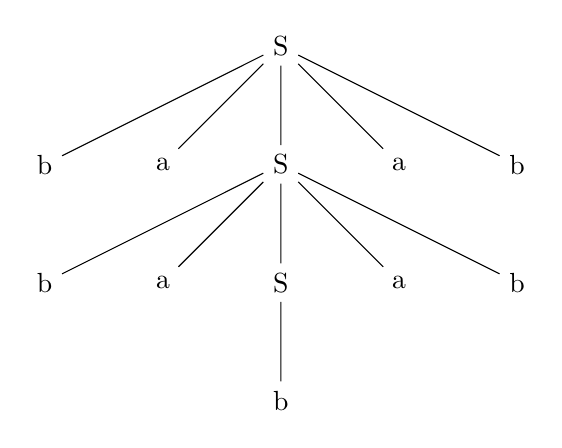
\begin{tikzpicture}
      [level 1/.style={sibling distance=15mm},
      level 2/.style={sibling distance=15mm},
      level 3/.style={sibling distance=15mm}]
      \node {S}
      child {
        node {b}
      }
      child {
        node {a}
      } 
      child {
        node{S}
        child {
          node {b}
        }
        child {
          node {a}
        }
        child {
          node{S}
          child {
            node {b}
          }
        }
        child {
          node {a}
        }
        child {
          node {b}
        }
      }
      child {
        node{a}
      }
      child {
        node{b}
      };
    \end{tikzpicture}
  \end{center}
  $S\Rightarrow baSab\Rightarrow babaSabab \Rightarrow babababab$
\end{frame}

\begin{frame}{Klausuraufgabe: WS 2015/16 A6}
  Gegeben sei die kontextfreie Grammatik $G=(\{S,A,B\},\{a,b\},S,P)$ mit der Produktionsmenge
  \begin{align*}
    P=\{S&\rightarrow ASB | A | B,\\
    A&\rightarrow Aa | \epsilon,\\
    B&\rightarrow bB | \epsilon\}.
  \end{align*}
  \begin{itemize}
    \item Geben Sie zwei verschiedene Ableitungsbäume der Grammatik für das Wort $aab$ an.
    \item Geben Sie einen regulären Ausdruck an, der die von $G$ erzeugte Sprache $L(G)$ beschreibt.
    \item Geben Sie eine kontextfreie Grammatik $G'$ an, die die Sprache $(L(G))^*$ erzeugt.
  \end{itemize}
\end{frame}

\begin{frame}{Klausuraufgabe: WS 2015/16 A6}
  \begin{align*}
    P=\{S&\rightarrow ASB | A | B,\\
    A&\rightarrow Aa | \epsilon,\\
    B&\rightarrow bB | \epsilon\}.
  \end{align*}
  Ableitungen für das Wort $aab$
  \begin{itemize}
    \pause
    \item $S\Rightarrow ASB \Rightarrow AAB\Rightarrow ...$
    \pause
    \item $S\Rightarrow ASB \Rightarrow AASBB\Rightarrow^2 A\epsilon S\epsilon B\Rightarrow ...$
  \end{itemize}
\end{frame}

\begin{frame}{Klausuraufgabe: WS 2015/16 A6}
  \begin{center}
    \begin{tikzpicture}
      [level 1/.style={sibling distance=15mm},
      level 2/.style={sibling distance=15mm},
      level 3/.style={sibling distance=15mm}]
      \node {S}
      child {
        node {A}
        child {
          node {A}
          child {
            node{$\epsilon$}
          }
        }
        child {
          node{a}
        }
      }
      child {
        node{S}
        child {
          node{A}
          child {
            node {A}
            child {
              node{$\epsilon$}
            }
          }
          child {
            node{a}
          }
        }
      }
      child {
        node{B}
        child {
          node{b}
        }
        child {
          node{B}
          child {
            node{$\epsilon$}
          }
        }
      };
    \end{tikzpicture}
  \end{center}
\end{frame}

\begin{frame}{Klausuraufgabe: WS 2015/16 A6}
  \begin{center}
    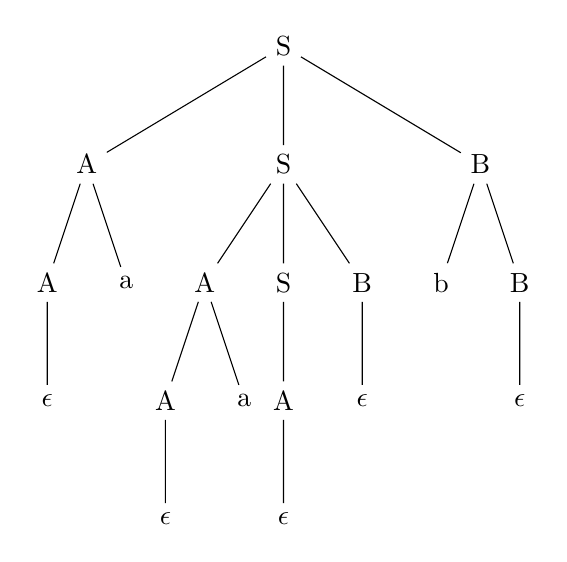
\begin{tikzpicture}
      [level 1/.style={sibling distance=25mm},
      level 2/.style={sibling distance=10mm},
      level 3/.style={sibling distance=10mm}]
      \node {S}
      child {
        node {A}
        child {
          node {A}
          child {
            node{$\epsilon$}
          }
        }
        child {
          node{a}
        }
      } 
      child {
        node{S}
        child {
          node{A}
          child {
            node {A}
            child {
              node{$\epsilon$}
            }
          }
          child {
            node{a}
          }
        }
        child {
          node{S}
          child {
            node{A}
            child {
              node{$\epsilon$}
            }
          }
        }
        child {
          node{B}
          child {
            node{$\epsilon$}
          }
        }
      }
      child {
        node{B}
        child {
          node{b}
        }
        child {
          node{B}
          child {
            node{$\epsilon$}
          }
        }
      };
    \end{tikzpicture}
  \end{center}
\end{frame}

\begin{frame}{Klausuraufgabe: WS 2015/16 A6}
  \begin{align*}
    P=\{S&\rightarrow ASB | A | B,\\
    A&\rightarrow Aa | \epsilon,\\
    B&\rightarrow bB | \epsilon\}.
  \end{align*}
  \begin{itemize}
    \item $L(G)=$\pause $\{a\}^*\{b\}^*$
    \pause
    \item $L(G)^*=\{a,b\}^*$
    \pause
    \item $G'=(\{S\},\{a,b\},S,\{S\rightarrow aS|bS|\epsilon\})$
  \end{itemize}
\end{frame}

